\documentclass[main.tex]{subfiles}
\ifxetex\else\onlyinsubfile{\usepackage{CJKutf8}}\fi
\begin{document}
\ifxetex\else\begin{CJK*}{UTF8}{song}\fi

\chapter{中断处理}
%% my chapter 1 content
%\onlyinsubfile{this only appears if chapter1.tex is compiled (not when main.tex is compiled)}
%\notinsubfile{this only appears if main.tex is compiled (not when chapter1.tex is compiled)}
%% more of my chapter 1 content
%%
\section{介绍}
ARM提供了7种运行模式,分别是user、system、supervisor、IRQ、FIQ、abort、undefined。除了user模式外,其他6种模式都是特权模式,如图\ref{figure:3-1}所示。

\begin{figure}[htp]
\centering
\includegraphics[scale=0.5]{figures/3-1.png}
\caption{ARM的7种模式}
\label{figure:3-1}
\end{figure}

\begin{itemize}
\item User : 唯一的非特权模式,用户程序运行在这种模式
\item System:与用户模式一样,只是属于特权模式
\item Supervisor:操作系统内核运行的模式,当CPU复位或swi指令执行时进入这种模式
\item IRQ :   当一个普通中断产生时将会进入这种模式
\item FIQ :   当一个快速中断产生时将会进入这种模式
\item Abort : 当CPU访问内存出现异常时将会进入这种模式
\item Undefined : 当CPU执行未定义指令时会进入这种模式
\end{itemize}

当ARM进入到异常模式时,它会跳转到从0开始的几个固定地址开始执行,这几个固定的地址称为异常向量表,如图\ref{figure:3-2}所示。该表共有8项,当CPU遇到异常,就会跳转到相对应的地址开始执行。

\par
本章主要关注的异常类型是IRQ。当外部设备触发中断时,ARM会把模式设置为IRQ模式,然后将pc设为0x18。此时,SPSR\_irq=CPSR,r14\_irq=(中断返回地址+4)。

\begin{figure}[htp]
\centering
\includegraphics[scale=0.35]{figures/3-2.png}
\caption{ARM的异常}
\label{figure:3-2}
\end{figure}

\section{扩充entry.S}
我们要对entry.S进行扩充以满足中断处理的需要。扩充的内容有以下三个方面:
\begin{itemize}
\item 填充异常向量表。
\item 初始化C语言中未初始化的全局或者静态变量。
\item 初始化各个CPU模式的栈。
\end{itemize}

首先来填充异常向量表,如代码\ref{code:3-1}所示。

\begin{code}
\captionof{listing}{chapter03/kernel/entry.S}
\label{code:3-1}
\inputminted[firstline=71,lastline=104,linenos,numbersep=5pt,frame=lines,framesep=2mm]{gas}{src/chapter03/kernel/entry.S}
\end{code}

可以看出,真正有效的只有reset和irq两项。因为kernel.img被加载到0x8000这个地址,从\_entry开始的异常向量表位于0x8000,而CPU希望异常向量表在0地址。因此,我们要把异常向量表从0x8000复制到0x0地址,才能保证异常的正常处理。复制异常向量表如代码\ref{code:3-2}所示。

\begin{code}
\captionof{listing}{chapter03/kernel/entry.S}
\label{code:3-2}
\inputminted[firstline=104,lastline=112,linenos,numbersep=5pt,frame=lines,framesep=2mm]{gas}{src/chapter03/kernel/entry.S}
\end{code}

在C语言中,要把未初始化的全局或静态变量全部置0。编译器会把这些变量统一放在一个称为BSS(Block Started by Symbol)的段中。在链接器脚本kernel.ld.in(代码\ref{code:2-5})中,我们定义的两个符号\_edata和\_end,分别标识了BSS段的开始和结束。在调用C程序之前,要确保这部分变量的值是0。这正是代码\ref{code:3-3}的功能。

\begin{code}
\captionof{listing}{chapter03/kernel/entry.S}
\label{code:3-3}
\inputminted[firstline=112,lastline=121,linenos,numbersep=5pt,frame=lines,framesep=2mm]{gas}{src/chapter03/kernel/entry.S}
\end{code}

接下来,为各个异常模式设置栈。记住,当前CPU正运行在supervisor模式。我们按照顺序先后为undefined、abort、IRQ和supervisor模式设置了栈。我们只给undefined、abort和IRQ的栈分配了12个字节。后面我们会看到,12个字节就够了。Supervisor的栈稍微大一点,从(0x1000-36)开始往0地址延伸。
\begin{code}
\captionof{listing}{chapter03/kernel/entry.S}
\label{code:3-4}
\inputminted[firstline=121,lastline=143,linenos,numbersep=5pt,frame=lines,framesep=2mm]{gas}{src/chapter03/kernel/entry.S}
\end{code}

在实际应用中,绝大部分代码运行在两种模式:user和supervisor模式。user模式用于运行用户应用程序,supervisor模式用于运行操作系统内核。
\par
当系统发生异常时,我们完成一些准备工作后,切换到supervisor模式,然后在supervisor模式下完成后续的流程。

\section{保存中断现场}
所谓中断现场(context),是指在中断发生前CPU的运行状态,即所有寄存器的值。前面讲过,当CPU被外部设备中断时,它会自动将pc=0x18,SPSR\_irq=CPSR,r14\_irq=(中断返回地址+4),其他寄存器仍然保持中断发生前的状态。因为在后续处理中断过程中可能会修改这些寄存器的值,我们必须完整地保存中断发生前CPU的运行状态,这个过程称为保存现场。当中断处理完成后,把这些保存的值恢复到寄存器中,CPU将以中断发生前的状态继续运行,即称为恢复现场。

\par
我们定义一个结构体来描述现场,它给出了中断发生时需要保存的寄存器。如代码\ref{code:3-5}所示。

\begin{code}
\captionof{listing}{chapter03/kernel/machdep.h}
\label{code:3-5}
\inputminted[firstline=25,lastline=45,linenos,numbersep=5pt,frame=lines,framesep=2mm]{c}{src/chapter03/kernel/machdep.h}
\end{code}

根据我们前面设置的异常向量表,中断发生时,CPU将跳转到irq开始执行。因为后面还会用到保存和恢复现场的代码,为了方便重用,我们把它们定义为宏,分别是PUSHCONTEXT和PULLCONTEXT。

\begin{code}
\captionof{listing}{chapter03/kernel/entry.S}
\label{code:3-6}
\inputminted[firstline=143,lastline=151,linenos,numbersep=5pt,frame=lines,framesep=2mm]{gas}{src/chapter03/kernel/entry.S}
\end{code}

此时sp指向IRQ模式的栈顶(即0x1000-24),(r14-4)保存了中断返回的地址,SPSR中保存了中断前的CPSR。我们先把返回地址(r14-4)存到栈上,即

\begin{code}
\captionof{listing}{chapter03/kernel/entry.S}
\label{code:3-7}
\inputminted[firstline=38,lastline=41,linenos,numbersep=5pt,frame=lines,framesep=2mm]{gas}{src/chapter03/kernel/entry.S}
\end{code}

保存lr之后,现在lr可以作为通用寄存器。因此,我们先把SPSR(即中断前的CPSR)也存到栈上。
\begin{code}
\captionof{listing}{chapter03/kernel/entry.S}
\label{code:3-8}
\inputminted[firstline=42,lastline=43,linenos,numbersep=5pt,frame=lines,framesep=2mm]{gas}{src/chapter03/kernel/entry.S}
\end{code}

至此,两个最重要的寄存器已经保存起来了。现在,我们要切换回supervisor模式去处理中断。问题是,我们切换到supervisor模式后,怎么才能记住IRQ模式栈的位置,将来才能从中取出中断返回地址和SPSR呢?为此,我们约定一个寄存器来保存IRQ模式栈的位置,而且这个通用寄存器不能受到模式切换的影响。为了简单起见,就用r0。因为我们不能修改r0的值,因此先把它存到IRQ模式栈上,然后让r0指向IRQ模式栈顶的位置。

\begin{code}
\captionof{listing}{chapter03/kernel/entry.S}
\label{code:3-9}
\inputminted[firstline=44,lastline=46,linenos,numbersep=5pt,frame=lines,framesep=2mm]{gas}{src/chapter03/kernel/entry.S}
\end{code}

特别要注意最后一条语句,它还原了IRQ模式栈的位置,以保证下次发生IRQ异常时,IRQ模式栈还是指向(0x1000-24)。因此,我们在IRQ模式栈上保存了中断返回地址、SPSR和r0,共12个字节。
\par
准备工作就绪,现在我们切换到supervisor模式。

\begin{code}
\captionof{listing}{chapter03/kernel/entry.S}
\label{code:3-10}
\inputminted[firstline=47,lastline=50,linenos,numbersep=5pt,frame=lines,framesep=2mm]{gas}{src/chapter03/kernel/entry.S}
\end{code}

此时,CPU已经运行在supervisor模式。我们把整个中断现场保存在supervisor模式栈中。首先为中断现场预留空间,然后把刚才保存在IRQ模式栈中的中断返回地址、SPSR和r0复制过来。

\begin{code}
\captionof{listing}{chapter03/kernel/entry.S}
\label{code:3-11}
\inputminted[firstline=51,lastline=57,linenos,numbersep=5pt,frame=lines,framesep=2mm]{gas}{src/chapter03/kernel/entry.S}
\end{code}

现在,可以保存中断发生时所有的寄存器。
\begin{code}
\captionof{listing}{chapter03/kernel/entry.S}
\label{code:3-12}
\inputminted[firstline=58,lastline=61,linenos,numbersep=5pt,frame=lines,framesep=2mm]{gas}{src/chapter03/kernel/entry.S}
\end{code}
至此,我们已经在supervisor模式栈上保存了现场,即struct context结构体,而且sp含有指向该结构体的指针。

\section{恢复中断现场}
当中断处理完成后,需要返回到被中断前的状态继续执行。相对于保存现场,恢复现场要简单一些。假设此时sp指向context结构体,直接用ldm指令恢复所有寄存器的值即可。

\begin{code}
\captionof{listing}{chapter03/kernel/entry.S}
\label{code:3-13}
\inputminted[firstline=63,lastline=69,linenos,numbersep=5pt,frame=lines,framesep=2mm]{gas}{src/chapter03/kernel/entry.S}
\end{code}

回到前面的irq。PUSHCONTEXT之后,调用C语言的中断处理程序irq\_handler,把现场context的指针当作参数通过r0寄存器传递给它。把中断现场传给中断处理函数,是考虑到在处理中断的过程中,可能需要了解中断发生时的状态信息。

\begin{code}
\captionof{listing}{chapter03/kernel/entry.S}
\label{code:3-14}
\inputminted[firstline=145,lastline=151,linenos,numbersep=5pt,frame=lines,framesep=2mm]{gas}{src/chapter03/kernel/entry.S}
\end{code}

下面我们来看irq\_handler,它的主要工作是判断哪个设备发生了中断,然后根据中断请求号码调用对应的中断处理函数。BCM2835有72个中断源,其中ARM侧的中断源8个,GPU侧64个,如图\ref{figure:3-3}和\ref{figure:3-4}所示。

\begin{figure}[htp]
\centering
\includegraphics[scale=0.4]{figures/3-3.png}
\caption{ARM侧中断源}
\label{figure:3-3}
\end{figure}

\begin{figure}[htp]
\centering
\includegraphics[scale=0.4]{figures/3-4.png}
\caption{GPU侧中断源}
\label{figure:3-4}
\end{figure}

我们按照先ARM、后GPU的顺序分配中断请求号码,即ARM Timer的中断请求号码是0,ARM Mailbox是1,Illegal access type 0是7,然后GPU的IRQ 0-63对应于8-71号。

\begin{code}
\captionof{listing}{chapter03/kernel/machdep.c}
\label{code:3-15}
\inputminted[firstline=83,lastline=117,linenos,numbersep=5pt,frame=lines,framesep=2mm]{c}{src/chapter03/kernel/machdep.c}
\end{code}

\noindent
其中g\_intr\_vector是中断向量表,一个包含了72个中断处理函数地址的数组。

\section{中断控制器}
中断控制器(Programmable Interrupt Controller, PIC)是计算机重要的设备之一,它负责汇集所有外部设备的中断,然后把中断信号发送给CPU,如图\ref{figure:3-5}所示。CPSR中的I位控制着CPU是否响应中断请求,而PIC控制着每个设备的中断请求。

\begin{figure}[htp]
\centering
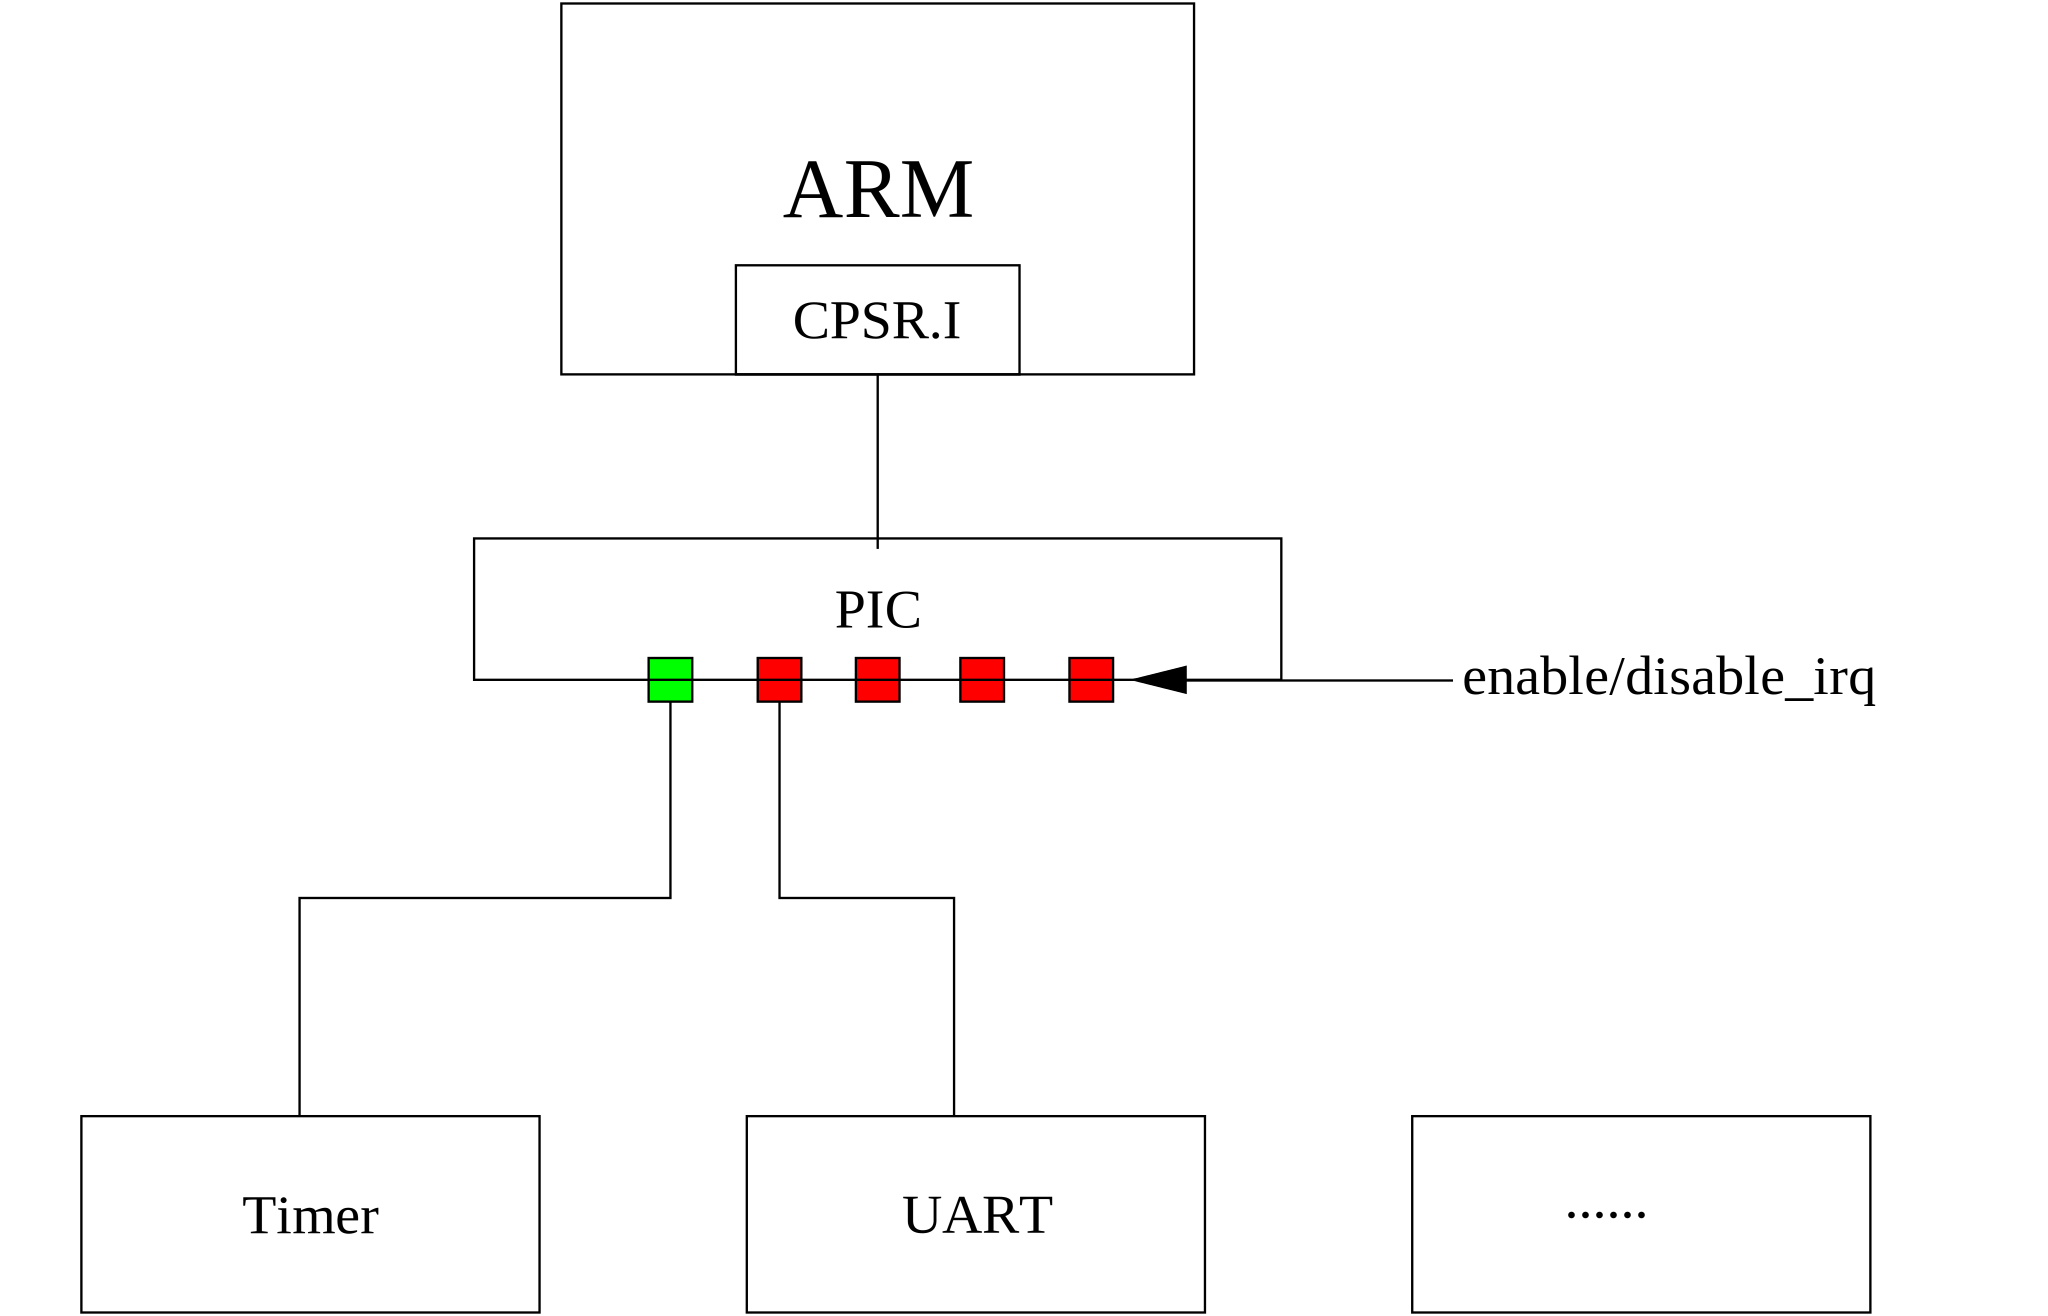
\includegraphics[scale=0.6]{figures/3-5}
\caption{中断控制器}
\label{figure:3-5}
\end{figure}

在系统启动过程中,要屏蔽所有设备的中断。这正是函数init\_pic做的工作。

\begin{code}
\captionof{listing}{chapter03/kernel/machdep.c}
\label{code:3-16}
\inputminted[firstline=42,lastline=51,linenos,numbersep=5pt,frame=lines,framesep=2mm]{c}{src/chapter03/kernel/machdep.c}
\end{code}

将来某个设备初始化完成后,再逐一打开它的中断。控制PIC中断开关的函数是enable\_irq和disable\_irq。

\begin{code}
\captionof{listing}{chapter03/kernel/machdep.c}
\label{code:3-17}
\inputminted[firstline=53,lastline=81,linenos,numbersep=5pt,frame=lines,framesep=2mm]{c}{src/chapter03/kernel/machdep.c}
\end{code}

\section{定时器中断}
可编程定时器(Programmable Interval Timer,PIT)是整个系统的脉搏,驱动着系统推进各项工作。具体来说,它有两个作用:维持时钟和实现分时调度。定时器的工作方式比较简单,就是以固定的频率中断CPU。

\par
BCM2835内部集成了一片定时器AP804,下面我们对它进行初始化。定时器发出中断的频率可以修改,初始化定时器的函数init\_pit的参数freq,就是需要的中断频率。

\begin{code}
\captionof{listing}{chapter03/kernel/machdep.c}
\label{code:3-18}
\inputminted[firstline=119,lastline=133,linenos,numbersep=5pt,frame=lines,framesep=2mm]{c}{src/chapter03/kernel/machdep.c}
\end{code}

下面来实现定时器的中断处理函数。首先,我们定义了一个全局变量g\_timer\_ticks记录定时器中断的次数。然后,为了验证定时器中断系统是否能工作,定时器中断一次,便往串口输出一个点。

\begin{code}
\captionof{listing}{chapter03/kernel/kernel.c}
\label{code:3-19}
\inputminted[firstline=3,lastline=23,linenos,numbersep=5pt,frame=lines,framesep=2mm]{c}{src/chapter03/kernel/kernel.c}
\end{code}

注意,在处理完中断后,要清除定时器的中断未决标志,表示本次中断处理完了,准备接收下一次中断。这个工作已经在irq\_handler中完成了,见代码\ref{code:3-15}中的110-115行。

\par
现在,我们已经完成各个模块的工作,可以在cstart函数中把它们组装起来。首先,初始化PIC和PIT,并把中断向量表填上默认的中断处理函数的地址。然后,把定时器中断处理函数的地址填入对应的中断向量表项,让PIC开启定时器中断。最后,因为CPU复位后默认不响应中断请求,即CPSR.I=1,我们用函数sti把CPSR.I=0,即让CPU响应中断请求。

\begin{code}
\captionof{listing}{chapter03/kernel/machdep.c}
\label{code:3-20}
\inputminted[firstline=135,lastline=166,linenos,numbersep=5pt,frame=lines,framesep=2mm]{c}{src/chapter03/kernel/machdep.c}
\end{code}

函数sti和对应的关闭中断请求函数cli定义在entry.S中,如代码\ref{code:3-20}所示。

\begin{code}
\captionof{listing}{chapter03/kernel/entry.S}
\label{code:3-21}
\inputminted[firstline=153,lastline=166,linenos,numbersep=5pt,frame=lines,framesep=2mm]{gas}{src/chapter03/kernel/entry.S}
\end{code}

好了,代码写完了,回到命令行敲make生成kernel.img,把kernel.img复制到SD卡,插入树莓派并打开电源,在串口输出中可以看到树莓派正在打点,如图\ref{figure:3-6}所示。这说明中断系统已经可以工作了。

\begin{figure}[htp]
\centering
\includegraphics[scale=0.5]{figures/3-6.png}
\caption{定时器中断的输出}
\label{figure:3-6}
\end{figure}

\clearpage
\ifxetex\else\end{CJK*}\fi
\end{document} 